\documentclass[11pt]{article}
\usepackage{graphicx}
\usepackage{cite}
\def\BibTeX{{\rm B\kern-.05em{\sc i\kern-.025em b}\kern-.08em
    T\kern-.1667em\lower.7ex\hbox{E}\kern-.125emX}}
\usepackage{url}
    \makeatletter
    \g@addto@macro{\UrlBreaks}{\UrlOrds}
    \makeatother
\usepackage{appendix}
\usepackage[version=3]{mhchem}
\usepackage{amsmath}
\usepackage{booktabs}
\usepackage{amssymb}
\usepackage{float}
\usepackage{commath}
\usepackage{siunitx}
\usepackage[a4paper,margin=20mm]{geometry}
\setlength{\parskip}{\baselineskip}%
\setlength{\parindent}{0pt}%
\sisetup{detect-all}
\begin{document}
\section*{Abstract}
\section*{Introduction}
\section*{Experimental setup and methodology}
\section*{Question 1}
\section*{Question 2}
\section*{Question 3}
The lower heating value is the amount of heat released in the complete combustion of a specific quantity of fuel at standard conditions (\SI{25}{\celsius} and \SI{1}{\bar}), without recovering the latent heat of vaporization from the water vapour content in the gaseous products CITATION. The LHV is preferred to HHV in relation to internal combustion engines as it is not practical to recover the energy contained in the gaseous water vapour in typical ICEs, as this would require cooling the combustion products until the water vapour condenses. In most engines the vapour is expelled from the system as part of the hot exhaust gases and is therefore unavailable to do useful work. 

Heating values may be determined using a calorimeter or derived empirically by considering an energy balance, as will be done here. The heating value of the renewable fuel, ethyl valerate (\ce{C7H14O2}), was estimated by considering its stoichiometric combustion in dry air. The chemical equation is presented as follows: 
\begin{equation}
    \ce{C7H14O2 + 9.5(O2 + 3.76N2) -> 7CO2 + 7H2O(g) + 35.72N2} \label{q3-1}
\end{equation}
Assuming perfect homogenous mixing of fuel and air, \SI{9.5}{\mol} of dry air (21\% oxygen and 79\% nitrogen by volume) is required per mole of fuel to achieve complete combustion. The heat released is therefore the difference between the enthalpies of the products and reactants CITATION.
\begin{equation}
    Q = \sum_P \left(n_i\overline{h_i}\right) - \sum_R \left(n_i\overline{h_i}\right) = H_P - H_R \label{q3-2}
\end{equation}
The enthalpy $\overline{h_i}$ at any state is a function of temperature and pressure, consists of the enthalpy of formation $h_f^{\ominus}$ at standard reference conditions and sensible enthalpy. For simplicity, only the enthalpy of formation was considered in the estimation as the exhaust temperatures are not known. This causes the heat release to be overestimated and leads to conservative results for thermal efficiency. 

According to the National Institute of Standards and Technology, the enthalpy of formation of the test fuel is $\Delta h_f^{\ominus} = \SI{-553}{\kilo\joule\per\mol}$ CITATION. $h_f^{\ominus}$ of the other compounds were obtained from property tables CITATION. From \eqref{q3-1} and \eqref{q3-2}, the LHB of ethyl valerate (\ce{C7H14O2}) is computed as follows:
\begin{equation}
    LHV_{\textrm{test}} = \left[-553.1-9.5\left(0+0\right)\right]-\left[7\left(-393.52\right)+7\left(-241.82\right)+35.72\left(0\right)\right] = \SI{3894.4}{\kilo\joule\per\mol}
\end{equation}
Taking the molecular weight of ethyl valerate to be \SI{130.185}{\kilo\gram\per\mole}, the LHV of the test fuel expressed in mass basis is: 
\begin{equation}
    LHV_{\ce{C7H14O2}} = \SI{29.91}{\mega\joule\per\kg}
\end{equation}
The LHV of the reference fossil gasoline is as provided: 
\begin{equation}
    LHV_{\textrm{G}} = \SI{42.7}{\mega\joule\per\kg}
\end{equation}
Therefore, the LHV of the fuel blend is the sum of the LHVs of the ethyl valerate and gasoline, weighted by mass fractions ($x_i$), which can be computed from their volume fractions ($v_i$) CITATION:
\begin{align}
    LHV_{\textrm{blend}} &= x_G \cdot \left(LHV\right)_G + x_{\ce{C7H14O2}} \cdot \left(LHV\right)_{\ce{C7H14O2}}\\
    x_G &= \frac{v_G \rho_G}{v_G \rho_G + v_{\ce{C7H14O2}}\rho_{\ce{C7H14O2}}}\\
    \therefore LHV_{\textrm{blend}} &= 0.88267\left(42.7\right) + \left(1-0.88267\right)\left(29.913\right) = \SI{41.20}{\mega\joule\per\kg}
\end{align}
The indicated specific fuel consumption ISFC is a measure of the amount of fuel used per unit of power output from the engine. It is given by the following equation CITATION:
\begin{equation}
    ISFC = \frac{\dot{m}_f}{\dot{W}} \label{q3-3}
\end{equation}
Where $\dot{m}_f$ is the mass flow rate of fuel and $\dot{W}$ is the power output. The power output of the engine may be derived from the indicated mean effective pressure IMEP calculated in Question 1, which is the average pressure required in the cylinder to produce the same amount of work throughout the 4 strokes. As IMEP does not factor friction losses, the power output is overestimated hence the actual fuel consumption is higher. The work done per power stroke is expressed as: 
\begin{equation}
    W_{\textrm{power}} = IMEP \times \textrm{Bore Area} \times \textrm{Stroke} = IMEP \times \textrm{Swept volume} \label{q3-4}
\end{equation}
The Ricardo E6 is a 4-stroke engine running at test conditions of 600 rpm, therefore there is 1 power stroke every 2 crankshaft rotations, i.e. 5 power strokes per second. The power output in \si{\kilo\watt} is:
\begin{equation}
    \dot{W} = 5\dot{W}_{power} \label{q3-5}
\end{equation}
The overall indicated thermal efficiency for the engine is by definition the useful work output over total heat input. It is a measure of how much of the fuel’s heating value is lost to incomplete combustion, heat loss to surroundings and friction, and other losses. Taking the cylinder to be the system, the heat input is simply the heat released during combustion within the cylinder, equal to mass flow rate of fuel times the fuel heating value. 
\begin{equation}
    \eta_{th} = \frac{\dot{W}}{\dot{Q}_{in}} = \frac{\dot{W}}{\dot{m}_f \times LHV_{\textrm{blend}}} \label{q3-6}
\end{equation}
Therefore, the efficiency and ISFC are related by the following: 
\begin{equation}
    \eta_{th} = \frac{1}{ISFC \times LHV_{\textrm{blend}}}
\end{equation}
Using the above relations, the calculated values for ISFC and indicated thermal efficiency for each spark timing are presented in Table \ref{q3-t1}, with the corresponding IMEP for reference. The thermal efficiencies were plotted against spark timing in Figure \ref{q3-f1}.
\begin{table}[H]
    \begin{center}
    \begin{tabular}{c c c c c}
        \toprule
        Fuel    & Spark time    & IMEP (\si{bar})   & Indicated specific fuel   & Indicated thermal \\
                & (deg BTDC)    &   & consumption (\si{\kg\per\joule})  & efficiency\\
        \midrule
        Reference   & 10    & 8.0096    & \SI{8.0218e-8}    & 0.292\\
        fossil      & 13    & 8.1568    & \SI{7.7742e-8}    & 0.302\\
        gasoline    & 16    & 8.1614    & \SI{7.8758e-8}    & 0.297\\
        \midrule
        10\% Ethyl  & 10    & 7.6880    & \SI{7.8958e-8}    & 0.307\\
        valerate    & 13    & 7.8622    & \SI{7.8158e-8}    & 0.311\\
                    & 16    & 7.9461    & \SI{7.6111e-8}    & 0.319\\
        \bottomrule
    \end{tabular}
    \caption{ISFC consumptions and indicated thermal efficiencies.}
    \label{q3-t1}
    \end{center}
\end{table}
\begin{figure}[H]
    \centering
    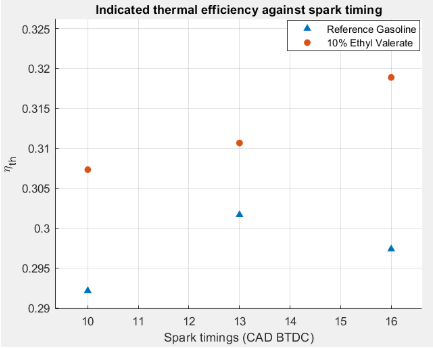
\includegraphics[height = 7cm]{./img/diagram1.png}
    \caption{Plot of indicated thermal efficiency against spark timing}
    \label{q3-f1}
\end{figure}
It is observed that thermal efficiency of the engine running on the fuel blend is higher than that of gasoline at all spark timings. Although the engine produces less work on the blend, the heat input requirements are also lower. 

The trend shows that in general, the indicated thermal efficiency increases with retarded spark timings. This is to be expected as earlier spark timings resulted in higher IMEPs, which translates to a higher indicated power output. Spark timings that are too advanced result in the gas expanding when the piston is already moving down from TDC, hence work done by the gas is not maximised. However, if the spark timing is too early, the gas expands against the piston when it is moving up towards TDC and it is not doing useful work. It has been determined experimentally that optimal power and efficiency for a spark ignition gasoline engine is achieved at 31 CAD BTDC (Zareei and Kakaee, 2013) CITATION. Therefore, for the range investigated in this experiment, an increase in indicated thermal efficiency with spark timing was expected to be observed.

For this reason, the efficiency for the gasoline fuel at 13 or 16 CAD BTDC was most likely to be anomalous as it does not fit with expectations of the trend. Although the IMEP showed a linear increase with later spark timings, the ISFC of the 13 CAD BTDC trial was significantly lower than 16 CAD BTDC. The reason for this anomaly can possibly be attributed to the measured fuel flow rate during test 4, which ranged from \SI{0.18}{\gram\per\second} at the beginning of the test to \SI{0.1}{\gram\per\second} by the end, giving a lower average fuel flow rate compared to the other two tests ran at the same spark timing. Since air mass flow rate remained relatively constant, and the methodology called for the air fuel ratio to remain constant throughout, this must be the result of an error, human or otherwise. This thus increased the average ISFC and thermal efficiency of the gasoline at 13 CAD BTDC. Removing the results of test 4 gives us a revised thermal efficiency closer to 29.6\%, which is much more reasonable given the expected trend. The revised thermal efficiencies with test 4 removed were plotted against spark timing in Figure \ref{q3-f2}. 
\begin{figure}[H]
    \centering
    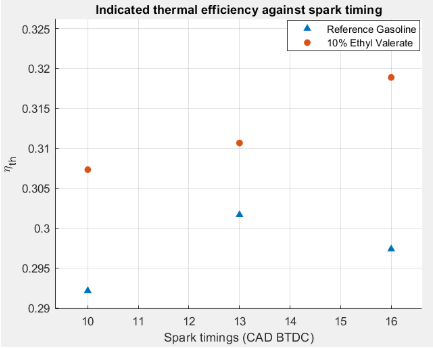
\includegraphics[height = 7cm]{./img/diagram1.png}
    \caption{Plot of indicated thermal efficiency with test 4 removed.}
    \label{q3-f2}
\end{figure}
In general, the LHV is an inaccurate estimate for heat input to the system. As mentioned previously the estimated LHV of the fuel blend overestimates the heat released in its combustion, hence the thermal efficiency is likely underestimated. Furthermore, using the product of fuel mass flow and LHV as $Q_{in}$ assumes that perfect combustion occurs, and the fuel is burnt completely. In reality, there will not be a homogenous mixture of air and fuel, hence there will be pockets of unburnt fuel that leave in the exhaust gases. In this manner, $Q_{in}$ is again overestimated.  

Additionally, as mentioned previously since the power output is an overestimate, since it was derived from the IMEP which this does not consider frictional losses which may occur in the moving parts of an ICE. Hence, the useful power will be lower in practical purposes and thus the thermal efficiencies calculated are also an overestimate. 

Lastly, it is important to consider whether it is appropriate to evaluate the system using thermodynamic analysis. Thermodynamic efficiency of the spark ignition engine is derived from the closed system analysis of the Otto cycle, whilst our experiment deals with a system that undergoes a mechanical cycle instead of a thermodynamic one. Though thermodynamic analysis is not strictly accurate with regards to our system, it is still useful for observing trends within our data. Our analysis allows us to conclude that efficiency increases with increased spark timings, and for all spark timings, the ethyl valerate fuel blend yields a higher thermal efficiency, meaning more energy is converted to useful work.  
\section*{Question 4}
\section*{Question 5}
\section*{Question 6}
\section*{Question 7}
\section*{Results and discussion}
\section*{Conclusions}
\begin{thebibliography}{00}

\end{thebibliography}
\end{document}